\documentclass[UTF8]{ctexart}

\usepackage{WeeklyReport}
\usepackage{graphicx}
\usepackage{amsmath}
\usepackage{amssymb}

\title{周报04}
\author{Jeff\ Fu}
\date{\today}

\begin{document}
    \maketitle
    % \tableofcontents
    \section{本周计划}
        \begin{itemize}
            \item 改进Partial Alignment Loss的代码并测试
        \end{itemize}
    \section{收获}
        上周实验的结果显示设计出的PAL效果并不理想,
        不过上周仅仅进行了很初步的训练(10 epoch以内),最终的PAL比较高(从100+下降到10左右)。
        进行了一些小改动之后,训练了100+个epoch,结果有很大提升。

        在原论文中给出的数据集里一共有5个domain,分别为mnist\_m、mnist、svhn、
        usps和synth\_number,其中mnist、usps和synth\_number在原论文中已取得
        接近90\%或更高的正确率,所以在进行PAL实验的时候,优先选择了正确率较低的
        mnist\_m和svhn。
        \subsection{mnist\_m测试结果(target为mnist\_m)}
            对原模型和添加了PAL的模型分别进行了训练。

            总共训练了102个epoch,在最后几个epoch中,原模型的正确率大概在72\%
            左右浮动(论文中给出的正确率是72.82\%),而添加了PAL之后,
            最后几个epoch的正确率达到了74\%左右,此时PAL已经明显降低(0.05左右)。

            训练中最后几个epoch的正确率如图 \ref{fig:mnistm} 所示。
            \begin{figure}[ht]
                \centering
                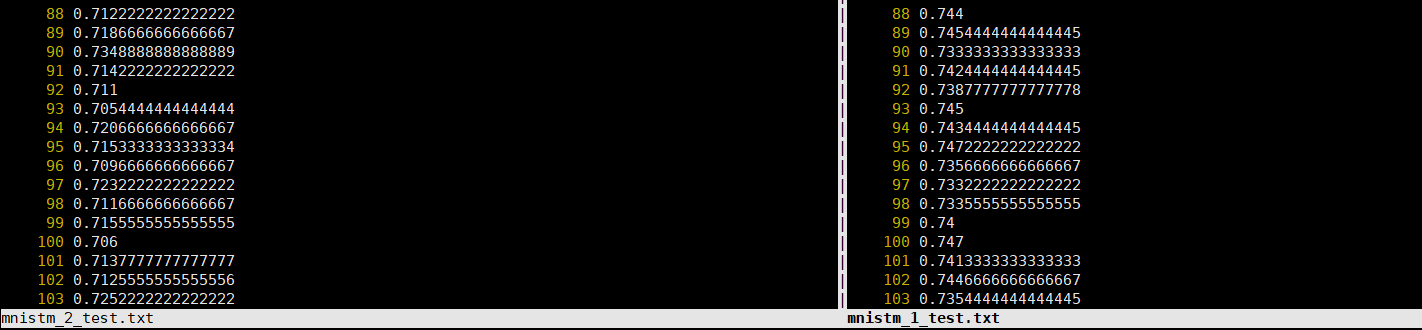
\includegraphics[scale=0.35]{Week04_mnistm.png}
                \caption{mnist\_m的训练结果,左边为原模型正确率,右边为添加PAL的模型的正确率}
                \label{fig:mnistm}
            \end{figure}
        \subsection{svhn测试结果(target为svhn)}
            同样也是对原模型和添加了PAL的模型分别进行训练,也是102个epoch。

            在最后几个epoch中,原模型的正确率大约有82\%(论文中给的正确率为81.32\%),
            而在添加了PAL的网络中,最后几个epoch的正确率在84\%附近。

            训练中最后几个epoch的正确率如 \ref{fig:svhn} 所示。
            \begin{figure}[ht]
                \centering
                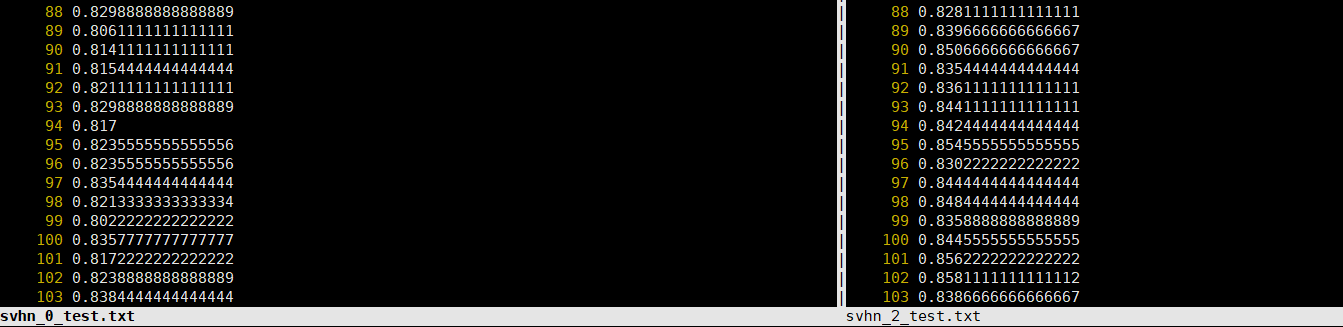
\includegraphics[scale=0.36]{Week04_svhn.png}
                \caption{svhn的训练结果,左边为原模型正确率,右边为添加PAL的模型的正确率}
                \label{fig:svhn}
            \end{figure}
        \subsection{分析}
            目前还不确定PAL正确率高是否是因为出现了over fitting,
            如果没有发生over fitting并且模型的实现无误的话,
            可以认为新增的PAL是有效的。

            值得一提的是,经过100+个epoch的训练之后,
            新旧模型的Loss已经很低(数量级在 $10^{-2}$ ),
            而添加了PAL之后,模型没有原先稳定,收敛速度也略慢了一些,
            不过在训练了100+ epoch之后也趋于稳定,整体正确率也比原模型高。

            另外,原模型在非常多的数据集(作者提出的DomainNet数据集和Digit Five)上进行了测试,
            这次我进行的测试只是其中一部分(Digit Five),结果可能带有一定的特殊性。
    \section{疑问/困难}
        我觉得差不多可以考虑用另外的数据进行测试了,或者把之前设想的NPN放进来试一试,
        但对于实验有一些不太清楚的地方:
        \begin{enumerate}
            \item 当前的代码基本上是在原代码的基础上删改而来的,特别是数据读取部分,
                使用了作者预处理好的数据,读取数据的代码也是直接使用了原代码,
                而这实际上导致了模型结构比较特殊,不方便与原先的一些benchmark进行比较
            \item 尽管当前取得了比原模型略好一些的结果,
                但是不知道如何科学地与其它模型进行比较(是否可以直接使用论文中给出的结果,
                或者说是否需要把别的模型按统一架构实现一遍再重新测试)
            \item 感觉仅仅使用一个PAL,与其它文章相比显得过于简陋了,
                正确率的提升也不是很明显(1\% $\sim$ 2\%)
        \end{enumerate}
\end{document}
